\documentclass[paper=letter, fontsize=11pt]{scrartcl}
\usepackage{comment}
\usepackage{graphicx}
\usepackage[T1]{fontenc}
\usepackage{fourier}
\usepackage[english]{babel}
\usepackage{amsmath,amsfonts,amsthm}
\usepackage{acronym}
\usepackage{listings}
\usepackage{sectsty}
\usepackage{fancyhdr}
\usepackage{geometry}
\geometry{margin=1in}
\pagestyle{fancyplain}
\allsectionsfont{\centering \normalfont\scshape}
\fancyhead{}
\fancyfoot[L]{}
\fancyfoot[C]{}
\fancyfoot[R]{\thepage}
\renewcommand{\headrulewidth}{0pt}
\renewcommand{\footrulewidth}{0pt}
\setlength{\headheight}{13.6pt}
\numberwithin{equation}{section}
\numberwithin{figure}{section}
\numberwithin{table}{section}
\setlength\parindent{0pt}
\newcommand{\horrule}[1]{\rule{\linewidth}{#1}}

\title{	
\normalfont \normalsize 
\textsc{University of Victoria, Computer Science Department} \\ [25pt]
\horrule{0.5pt} \\[0.4cm]
\huge CSC-586A Self-Adaptive Systems\
\horrule{2pt} \\[0.5cm]
}

\author{Tory Borsboom, Sean Debroni, Stephan Heinemann}
\date{\normalsize\today}

\begin{document}
\maketitle 

\small
\clearpage
\section{Part III -- Sensor APIs}
\label{sec:part3}

\subsection{Android Sensor API}
\label{sec:android_sensor_api}
\par
Android devices have a wide variety of sensors available to them, of both the
hardware and software variety. For Android, hardware sensors are physical
components build into the Android device, while software sensors are built on
top of one or more hardware sensors, and interpret their data in a more useful
fashion. Sensors for Android devices usually fall into one of these three
categories: motion sensors, environmental sensors, and position sensors.
\newline

\par
The Sensor \ac{API} for Android consists of four main classes and interfaces:
\texttt{SensorManager}, \texttt{Sensor}, \texttt{SensorEventListener}, and
\texttt{SensorEvent}.
\newline

\par
The \texttt{SensorManager} class is used to access a device's sensors. The
following code demonstrates the instantiation of this class:

\begin{lstlisting}[basicstyle=\small,language=Java]
	SensorManager sm = (SensorManager) getSystemService(Context.SENSOR_SERVICE);
\end{lstlisting}

\par
The \texttt{Sensor} class represents one of the device's sensors. Each sensor
has a unique type, which is used to get an instance of that sensor.
For example, to get a gyroscope sensor instance, the following code snippet
is used:

\begin{lstlisting}[basicstyle=\small,language=Java]
	Sensor s =  sm.getDefaultSensor(Sensor.TYPE_GYROSCOPE);
\end{lstlisting}

\par
\texttt{SensorEventListener} is an interface that contains two listener
methods to be implemented by the user:
%\texttt{onSensorChanged(SensorEvent event)},
%\texttt{onAccuracyChanged(Sensor sensor, int accuracy)}.

\begin{lstlisting}[basicstyle=\small,language=Java]
	onSensorChanged(SensorEvent event)
	onAccuracyChanged(Sensor sensor, int accuracy)
\end{lstlisting}

\par
Assuming an implementation of \texttt{SensorEventListener} in a class called
\texttt{My\-Sen\-sor\-Event\-List\-ener}, for the gyroscope sensor, its
registration code would look like this:

\begin{lstlisting}[basicstyle=\small,language=Java]
	MySensorEventListener msel = new MySensorEventListener();
	sm.registerListener(msel, s, SensorManager.SENSOR_DELAY_UI);
\end{lstlisting}

\par
\texttt{SENSOR\_DELAY\_UI} is one of four different delay settings, measured in
microseconds, that controls how often \texttt{onSensorChanged} listener method
is called.
These are, in order of fastest to slowest,
\texttt{SENSOR\_DELAY\_FASTEST}, \texttt{SENSOR\_DELAY\_GAME},
\texttt{SENSOR\_DELAY\_NORMAL}, and \texttt{SEN\-SOR\_\-DE\-LAY\_\-UI}. This
timing is just a hint to the system, events may be received faster or slower than the
specified rate. From Android $2.3$ onwards, any delay in microseconds can be
specified, not just these four constants.
\newline

\par
A \texttt{SensorEvent} consists of four fields -- the accuracy of the event,
which sensor generated the event, a timestamp indicating the time in
nanoseconds that the event occurred at, and a float array of values, whose
length and contents depends upon the type of sensor being monitored. For the
gyroscope sensor, this float array contains three values, the angular speed
around the $x$, $y$, and $z$ axis' in radians/second.
\newline

\par
The Android Sensor \ac{API} consists of these four classes and interfaces; it
does not matter what sensor is being monitored, the only thing that changes is
the implementation of \texttt{on\-Sen\-sor\-Changed} and
\texttt{onAccuracyChanged}.
This is a very nice generic interface for Sensors.\footnote{All information is
sourced from the Android documentation:\\
developer.android.com/guide/topics/sensors/sensors\_overview.html}

\subsection{iOS Magnetic Compass API}
\label{sec:ios_compass_api}
\par
The {\em iOS}\footnote{https://www.apple.com/ca/ios/what-is/} platform used on
{\em Apple}\footnote{https://www.apple.com} phones and tablets supports a
variety of motion services via an object called \texttt{CMMotionManager}. This
object is the gateway to raw {\em accelerometer}, {\em gyroscope} and
{\em magnetometer} data, as well as some processed data such as {\em rotation
rate}, {\em attitude}, {\em calibrated magnetic fields},
{\em direction of gravity}, and the {\em direction of acceleration} of the
device.
Of particular interest here, however, is the magnetometer and how the device
handles the data collected by this sensor.
\newline

\par
The magnetometer in the device collects magnetic field data, such as strength
and polarity, which is accessible via the \texttt{CMMotionManager} object
discussed above by either setting an interval at which updates can be pushed,
or by polling the sensor whenever an update is required. If requesting updates
at intervals the \texttt{accelero\-me\-ter\-Up\-date\-Inter\-val} property must
be specified and the \texttt{startMagnetometerUpdatesToQueue:withHandler:} method is called
which requires a \texttt{CMMagnetometerHandler} type object to be passed into
it.
This method will add data to a queue which can then be processed as needed.
The alternative to requesting repeated information at intervals is periodic
sampling of the data which is performed by calling
\texttt{startMagnetometerUpdates} and then simply reading
the \texttt{magnetomerData} property. For both of these methods it
is important that the \texttt{stopMagnetometerUpdates} method is called when
the system no longer needs to process magnetometer data. 
\newline

\par
In order to access the data acquired from the most recent polling of the
sensor, \texttt{mag\-neto\-me\-ter\-Da\-ta} must be accessed, this property is a
structure of type \texttt{CMMagnetometerData}. It contains three \texttt{int} values $x$, $y$, and
$z$. These \texttt{int} values represent the directional magnetic field relative
to the body of the device in microteslas. In the
coordinate system used, the $z$ axis is positive up through the front of the
screen, the $y$ axis is positive up through the top of the phone, and the $x$
axis is positive to the right of the device if the screen is facing the user.
There are also two methods made for simply polling the sensor to see if it is
working or available: \texttt{magnetometerActive} and
\texttt{magnetometerAvailable}. The method \texttt{magnetometerActive} checks
to see if the sensor is currently taking readings and
\texttt{magnetometerAvailable} checks to see if the sensor is available for
use.
\newline

\par
The purpose of having the two separate collection methods is one of resource
management. If the purpose of the app being written is something like a game or
some sort of mapping software, it is unnecessary to acquire data rapidly and
keep it in a queue. Most programs intended for light users will simply need to
query the sensor once per frame rendered on the screen at the very most. The
only time it would be necessary to use the queuing method is if the data needs
to be incredibly precise and with little latency between updates, such as if
the device were being used as a magnetometer in an experiment measuring
magnetic flux.
\newline

\subsection{NuttX / ArduPilot PX4 Optical Flow and Sonar API}
\label{sec:ardupilot_flow_api}
\lstset{language=C++}
\par
The {\em ArduPilot}\footnote{http://ardupilot.com/} autopilot stack supports a
wide range of sensors to be used with any of the supported vehicle types
including {\em Plane}, {\em Copter} and {\em Rover}. It builds on top of the
{\em NuttX}\footnote{http://nuttx.org/} operating system and requires the
applicable firmware for the underlying hardware such as the
{\em Pixhawk}\footnote{https://pixhawk.org} autopilot module.
\newline

\par
The supported sensor types include those to capture data about the vehicle's
{\em environment} as well as those related to its own {\em capabilities} in
order to establish an adequate {\em situational awareness}.
Supported environmental sensors gather {\em inertial} (attitude and
acceleration), {\em barometric} (altitude and airspeed), {\em magnetic}
(direction), {\em range} (distance), {\em optical} (orientation and recognition)
and {\em satellite} (position) data. Sensors that capture the vehicle's
capability state include a {\em battery monitor} (power consumption and
endurance) and a {\em performance monitor} (scheduler latency). Environmental
sensors themselves may provide self-reflective {\em health} and {\em quality}
monitoring functions. Furthermore, all information that is provided by the {\em NuttX}
operating system about its {\em Pixhawk} platform including the available
{\em memory} and {\em filesystem} space can be instrumented to enhance the
vehicle's capability state.
\newline

\par
The {ArduPilot} \ac{API} separates sensor {\em frontends} (interfaces) from
their actual {\em backends} (implementations) in order to easily support
different sensors of the same class. These sensors and other \ac{HAL} modules
can be found in the \texttt{libraries}
directory\footnote{https://github.com/diydrones/ardupilot} and are, hence,
separate from any concrete vehicle-related software. The {\em Copter} vehicle
employs the sensor \ac{API} through its \texttt{sensors.pde} arduino sketch
file which represents an even higher level
\ac{API}\footnote{http://www.arduino.cc/en/pmwiki.php?n=Reference/HomePage}
to the actual vehicle functions such as different autoflight modes.
\newline

\par
As a representative example, the structure of the {\em PX$4$ Optical Flow /
Sonar}\footnote{https://pixhawk.org/modules/px4flow} sensor interface shall be
explained. It is connected to the {\em Pixhawk} autopilot module as shown in
Figure \ref{fig:pixhawk_px4_flow_connection}.

\par
This sensor allows capturing the optical flow, that is, the rate of
translational and rotational changes in a captured image, in order to establish
positional information. The optical flow camera is mounted on the bottom of the
{\em Iris}\footnote{http://3drobotics.com/iris/} quadcopter body pointing
downwards and sampling the floor pattern that is being overflown. Since the
aircraft can be tilted (pitch and bank) and flown at different altitudes, a
range finder (sonar sensor) on the same sensor board is employed to relate the
optical flow information to the measured ground distances accordingly. Assuming
the actual attitude of the aircraft based on inertial sensors is known, an
actual ground distance can be derived from the sonar slant range readings.
\newline

\par
Figure \ref{fig:optical_flow_api} shows a small extract of the optical flow
sensor frontend \ac{API} in the \texttt{libraries/} \texttt{AP\_OpticalFlow}
directory possessing the sensor state data structure as well as methods that determine
flow and body rates in a two-dimensional image. The interface itself
furthermore consists of methods that determine the health of the sensor and the
quality of the data being captured by it.
\newline

\par
Figure \ref{fig:range_finder_api} shows an \ac{API} extract of the range finder
component of the optical flow sensor board. On the {\em PX$4$ Optical Flow}
board, a sonar sensor is employed to obtain range in order to relate optical
flow to ground distance. This concrete implementation is abstracted by the
more generic range finder \ac{API} in the \texttt{libraries/AP\_RangeFinder}
directory.
\newline

\par
The \texttt{sensors.pde} arduino sketch file uses the above \ac{API} in order
to provide the {\em Copter} vehicle with necessary sensor data to perform its
functions such as automatic flight modes. The overall static structure is shown
in Figure \ref{fig:of_sensor_board_api}.
\newline

\subsection{Application Example}
\label{sec:application_example}
\par
A small application example makes use of the {\em PX$4$ Optical Flow} board
connected to the {\em Iris} {\em Pixhawk} autopilot module. This application
realizes a flight envelope warning alert. The alert is triggered whenever
translational flow or rotational body rates exceed a certain limit. It is
also triggered when the \ac{AHRS}\footnote{
http://en.wikipedia.org/wiki/Attitude\_and\_heading\_reference\_system}
which fuses different sensor inputs for the current height of the aircraft
including the sonar distance reports a height above ground that exceeds a
certain threshold.
\newline

\par
The alert consist a series of high pitch tones whenever the normal envelope
is violated and a long low pitch tone as soon as the normal flight envelope
is re-established. Furthermore, the aircraft status \ac{LED} continues to
flash red as long as the normal envelope is violated. Snippets of the
documented application code can be found in the Appendix \ref{figures}.

\subsection{Application in the Cloud}
\label{sec:application_cloud}
\par
The optical flow sensor can be used to establish position and, hence, to
support higher-level autopilot modes such as loitering and following a
sequence of legs between waypoints. It can be fused with other sensor data
and provide a higher degree of redundancy. The tracks and sensor data of
small \acp{UAV} can be shared in the cloud. Such an existing project is
called {\em Droneshare}\footnote{http://www.droneshare.com/}. Having access
to and being able to mine shared mission data enables more
efficient planning and execution of coordinated missions that involve
multiple \acp{UAV}. Examples of coordinated missions include {\em aerial
surveillance}, {\em crop spraying} and {\em search and rescue} among many
other applications. Sharing position and altitude of \acp{UAV} can also
be used for enforcing compliance with airspace restrictions.

\clearpage
\label{appendix}
\section{Figures}
\label{figures}

\begin{figure}[h]
	\centering
    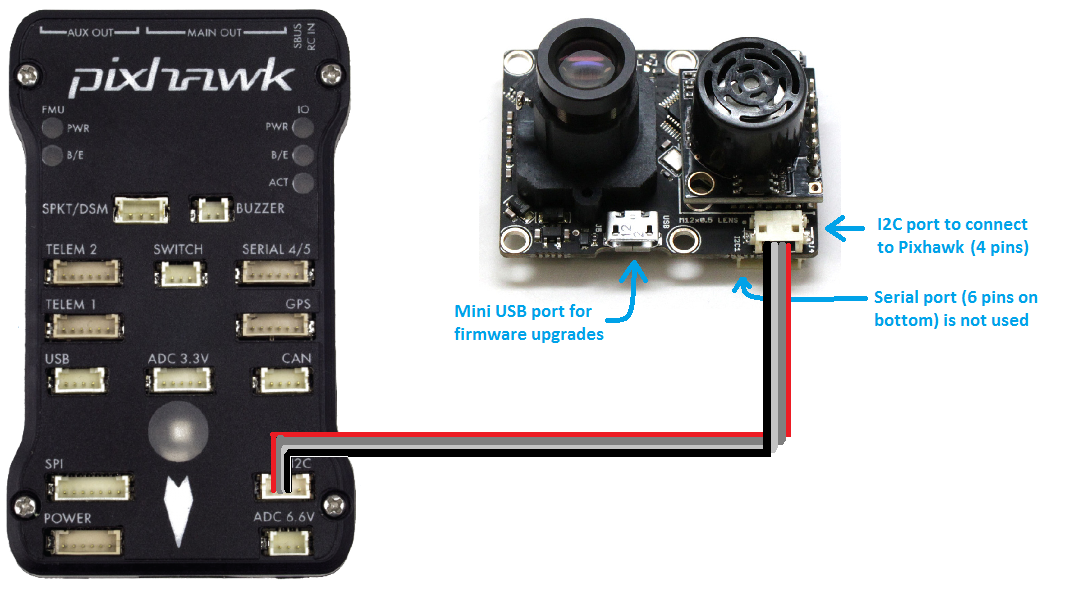
\includegraphics[width=300px]{graphics/PixhawkPX4Flow.png}
	\caption{Pixhawk PX4 Flow Connection}
	\label{fig:pixhawk_px4_flow_connection}
\end{figure}

\begin{figure}[h]
	\begin{lstlisting}[basicstyle=\scriptsize]
class OpticalFlow { //...
public: //...
	bool enabled() const { return _enabled; }
	bool healthy() const { return backend != NULL && _flags.healthy; }
	uint8_t quality() const { return _state.surface_quality; }
	const Vector2f& flowRate() const { return _state.flowRate; }
	const Vector2f& bodyRate() const { return _state.bodyRate; }
	uint8_t device_id() const { return _state.device_id; }
    //...
    struct OpticalFlow_state {
    	uint8_t device_id;
    	uint8_t  surface_quality;
    	Vector2f flowRate;
    	Vector2f bodyRate;
    };
private: //...
};
	\end{lstlisting}
	\caption{Optical Flow Sensor \ac{API}}
	\label{fig:optical_flow_api}
\end{figure}

\begin{figure}[h]
	\begin{lstlisting}[basicstyle=\scriptsize]
class RangeFinder {
public: //...
	enum RangeFinder_Status {
		RangeFinder_NotConnected = 0,
		RangeFinder_NoData,
		RangeFinder_OutOfRangeLow,
		RangeFinder_OutOfRangeHigh,
		RangeFinder_Good
	};
	
	struct RangeFinder_State {
		uint8_t instance;
		uint16_t distance_cm;
		uint16_t voltage_mv;
		enum RangeFinder_Status status;
		uint8_t range_valid_count;
		bool pre_arm_check;
		uint16_t pre_arm_distance_min;
		uint16_t pre_arm_distance_max;
	};
	//...
	uint16_t distance_cm() const { return distance_cm(primary_instance); }
	uint16_t voltage_mv() const { return voltage_mv(primary_instance); }
	int16_t ground_clearance_cm() const { return _ground_clearance_cm[primary_instance]; }
	RangeFinder_Status status(void) const { return status(primary_instance);
	//...
private: //...
};
	\end{lstlisting}
	\caption{Range Finder \ac{API}}
	\label{fig:range_finder_api}
\end{figure}

\begin{figure}[h]
	\centering
    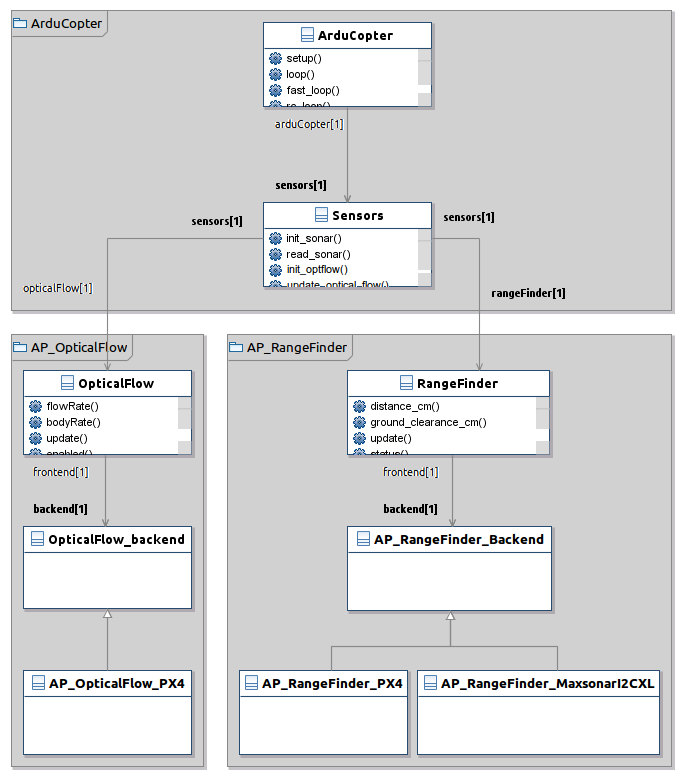
\includegraphics[width=400px]{graphics/OpticalFlowDiagram.png}
	\caption{PX4 Optical Flow Sensor Board \ac{API}}
	\label{fig:of_sensor_board_api}
\end{figure}

\begin{figure}[h]
	\begin{lstlisting}[basicstyle=\scriptsize]
static void stabilize_run()
{
    //...
    // in the stabilizing flight mode check the current flight envelope
    // measured by the optical flow sensor
    checkEnvelope();
    //...
}

#define BODY_RATE_ENVELOPE 4.0f
#define FLOW_RATE_ENVELOPE 1.0f
#define MAX_ALT 1.0f

static bool checkBodyRateEnvelope() {
        Vector2f bodyRate = optflow.bodyRate();
        return ((bodyRate.x > -BODY_RATE_ENVELOPE) && (bodyRate.y < BODY_RATE_ENVELOPE));
}

static bool checkFlowRateEnvelope() {
        Vector2f flowRate = optflow.flowRate();
        return ((flowRate.x > -FLOW_RATE_ENVELOPE) && (flowRate.y < FLOW_RATE_ENVELOPE));
}

static bool checkAltitudeEnvelope() {
        float hagl = 0.0f;
        ahrs.get_NavEKF().getHAGL(hagl);
        return (hagl <= MAX_ALT);
}

static void checkEnvelope() {
        // if the flight envelope is violated, then notify an envelope alert
        // notification subscribers include the tone alert and LED
        if (!checkBodyRateEnvelope() || !checkFlowRateEnvelope() || !checkAltitudeEnvelope()) {
                hal.console->printf("envelope violated\n");
                AP_Notify::flags.envelope_alert = true;
        } else {
                hal.console->printf("envelope satisfied\n");
                AP_Notify::flags.envelope_alert = false;
        }
}
	\end{lstlisting}
	\caption{Application Snippets}
	\label{fig:application_snippets}
\end{figure}

\clearpage
\section{Acronyms}
\label{acronyms}

\begin{acronym}
	\acro{AHRS}{Attitude and Heading Reference System}\\
		An attitude and heading reference system consists of sensors on
		three axes that provide attitude information for aircraft, including
		heading, pitch and yaw.They are designed to replace traditional
		mechanical gyroscopic flight instruments and provide superior
		reliability and accuracy.
		\footnote{http://en.wikipedia.org/wiki/Attitude\_and\_heading\_reference\_system}
	\acro{API}{Application Programming Interface}\\
		In computer programming, an application programming interface is a set
		of routines, protocols, and tools for building software applications.
		An API expresses a software component in terms of its operations,
		inputs, outputs, and underlying types. An API defines functionalities
		that are independent of their respective implementations, which allows
		definitions and implementations to vary without compromising each
		other.
		\footnote{http://en.wikipedia.org/wiki/Application\_programming\_interface}
	\acro{CPS}{Cyber-Physical System}\\
		A cyber-physical system is a system of collaborating computational
		elements controlling physical entities. Today, a precursor generation
		of cyber-physical systems can be found in areas as diverse as
		aerospace, automotive, chemical processes, civil infrastructure,
		energy, healthcare, manufacturing, transportation, entertainment, and
		consumer appliances.
		\footnote{http://en.wikipedia.org/wiki/Cyber-physical\_system}
	\acro{HAL}{Hardware Abstraction Layer}\\
		Hardware abstractions are sets of routines in software that emulate
		some platform-specific details, giving programs direct access to the
		hardware resources.
		\footnote{http://en.wikipedia.org/wiki/Hardware\_abstraction}
	\acro{II}{Industrial Internet}\\
		The Industrial Internet refers to the integration of complex physical
		machinery with networked sensors and software.
		\footnote{http://en.wikipedia.org/wiki/Industrial\_Internet}
	\acro{IIoT}{Industrial Internet of Things}\\
		The Industrial Internet of Things is a subdiscipline of the \acs{IoT},
		which describes IP-enabled systems in factories, offices and other
		commercial (and sometimes government) facilities. It is the part of the
		\acs{IoT} that focuses on how smart machines, networked sensors and
		sensor analytics can help improve business-to-business initiatives
		across a wide variety of industries, especially manufacturing.
		\footnote{http://itlaw.wikia.com/wiki/Industrial\_Internet\_of\_Things}
	\acro{IoT}{Internet of Things}\\
		The Internet of Things is the network of physical objects or "things"
		embedded with electronics, software, sensors and connectivity to enable
		it to achieve greater value and service by exchanging data with the
		manufacturer, operator and/or other connected devices.
		\footnote{http://en.wikipedia.org/wiki/Internet\_of\_Things}
	\acro{LED}{Light-Emitting Diode}
		A light-emitting diode is a two-lead semiconductor light source. It is
		a pn-junction diode, which emits light when activated. When a suitable
		voltage is applied to the leads, electrons are able to recombine with
		electron holes within the device, releasing energy in the form of
		photons.
		\footnote{http://en.wikipedia.org/wiki/Light-emitting\_diode}
	\acro{SoSs}{System of Systems}\\
		System of systems is a collection of task-oriented or dedicated systems
		that pool their resources and capabilities together to create a new,
		more complex system which offers more functionality and performance
		than simply the sum of the constituent systems.
		\footnote{http://en.wikipedia.org/wiki/System\_of\_systems}
	\acro{ToE}{Theory of Everything}\\
		A theory of everything or final theory, ultimate theory, or master
		theory is a hypothetical single, all-encompassing, coherent theoretical
		framework of physics that fully explains and links together all
		physical aspects of the universe.
		\footnote{http://en.wikipedia.org/wiki/Theory\_of\_everything}
	\acro{UAV}{Unmanned Aerial Vehicle}\\
		An unmanned aerial vehicle, known in the mainstream as a drone and also
		referred to as an unpiloted aerial vehicle and a remotely piloted
		aircraft by the International Civil Aviation Organization, is an
		aircraft without a human pilot aboard.
		\footnote{http://en.wikipedia.org/wiki/Unmanned\_aerial\_vehicle}
	\acro{ULSS}{Ulta-Large-Scale System}\\
		Ultra-large-scale system is a term used in fields including Computer
		Science, Software Engineering and Systems Engineering to refer to
		software intensive systems with unprecedented amounts of hardware,
		lines of source code, numbers of users, and volumes of data.
		\footnote{http://en.wikipedia.org/wiki/Ultra-large-scale\_systems}
\end{acronym}

\clearpage
\label{bibliography}
\bibliographystyle{plain}
\bibliography{csc-586a-13}

\end{document}